%
% Chapter 3
%
\chapter{PDP vs. Conventional Display Protocols}
\section{DVI \& HDMI}
Early scene generators used the DVI protocol, which is a simple and well understood standard. Unfortunately, they are also quite large connectors that did not fit well into the CSE design. For this reason, HDMI was chosen as the display protocol for NUCPC to CSE. HDMI uses the same electrical levels as DVI which kept it compatible with preexisting scene generator technology. \par
While they are good solutions, these display protocols are also rather limited. They are forced to remain compatible with even older protocols such as VGA. An example of typical display function is shown below. Video data is sent in sequential horizontal lines. Once the boundary of the display is reached, a "blanking period" is entered to reset the device's row/frame. The blanking period is recognized by a sync signal, which means that bandwidth and time are required for non-video data. If blanking periods were able to be reduced, it would inversely increase the potential frame rate. \par
Fixed frame-rate display protocols are also inherently limited. If a new frame is not necessary, the last frame will be retransmitted. Bandwidth is static which is useful for the reliability of consumer products, but less useful for a high-speed infrared projector. As such, utilizing the potential bandwidth of HDMI became a top priority and the foundation for the CSE firmware.
\begin{figure}[!htb]
	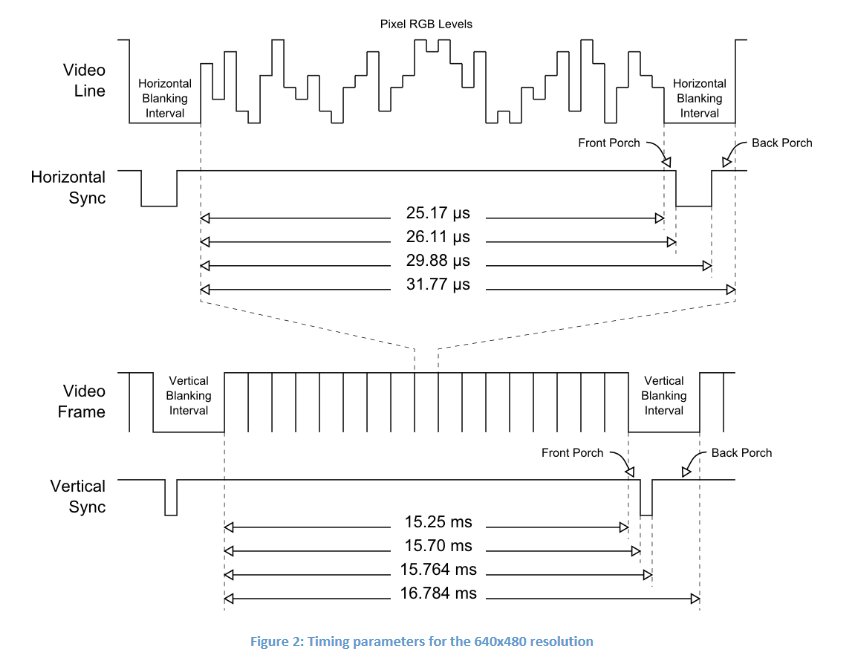
\includegraphics[width=\textwidth]{altera_vga.png}
	\centering
	\caption{VGA display protocol timing diagram \cite{alteravga}}
	\centering
\end{figure}
\section{PDP}
The Packetized Display Protocol (PDP) is the communication protocol for the CSE to LED array. The initial vision for PDP consisted of a "physical layer agnostic method of pixel data transmission capable of providing and addressing latency guarantees while maximizing bandwidth utilization" \cite{pdp_ieee}. Unlike traditional display communication protocols, PDP does not operate on entire display frames, and instead splits any projected scene into regions known as sub-frames. These sub-frames can be written to individually, greatly increasing bandwidth utilization and allowing for high frame rates beyond any traditional HDMI connection. \par
Sub-frames are marked by the PDP firmware with packets denoting their x and y coordinates. PDP communication packets will then consist of a packet header for draw location followed by the desired data. This divide-and-conquer strategy allows the NUCPC to only send frames when they require updates and therefore update relevant subframes at much higher frame rates than normally possible \cite{chris}. IRSP is an incredible application for this concept, as many scenes only have small regions that require updates. An example scene may contain a subframe changing at 200Hz, another at 50Hz, and yet another remaining static. Over a traditional display protocol, displaying any of these regions at the appropriate rates would be impossible due to the entire frames being sent at preset intervals. PDP, however, allows the NUCPC to utilize far more HDMI bandwidth to only send packets relevant to the subframes.\par
\begin{figure}[!htb]
	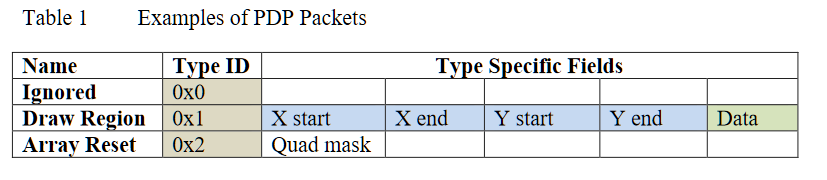
\includegraphics[width=10cm]{pdp_table.png}
	\centering
	\caption{Example PDP Packet \cite{chris}}
	\centering
\end{figure}
PDP can be used in two modes. The method of splitting and refreshing subframes is known as "streaming mode". Users may also opt to use it in a typical display mode where the entire frame is sent at a fixed refresh rate. This is known as "backwards compatibility mode". While there is nothing innovative about this mode, it is necessary to maintain compatibility with existing scene generation technology.\par
PDP was previously described as being "physical layer agnostic" \cite{pdp_ieee}. The protocol can theoretically be implemented over any physical medium such as DVI or ethernet. The initial implementation utilized HDMI to maintain compatiblity with existing technology, but a future revision is moving the physical medium to SFP+. Improvements to the CSE hardware will be briefly discussed in a later section.